\documentclass[11pt,a4paper]{article}
\usepackage[T1]{fontenc}
\usepackage[utf8]{inputenc}
\usepackage{lmodern,microtype}
\usepackage[margin=25mm]{geometry}
\usepackage{amsmath,amssymb,amsthm,booktabs,tikz,array}
\usetikzlibrary{arrows.meta,positioning}
\usepackage{xcolor}
\definecolor{inkplum}{HTML}{573354}
\definecolor{inkteal}{HTML}{236B70}
\usepackage{hyperref}
\hypersetup{colorlinks=true,linkcolor=inkplum,citecolor=inkplum,urlcolor=inkteal,
 pdftitle={Linear coordinate presentations of Lotka--Volterra tree systems and a proof of van der Kamp's tree conjecture},pdfauthor={Anonymous}}
\usepackage{fancyhdr}
\pagestyle{fancy}\fancyhf{}
\fancyhead[L]{\small Lotka--Volterra tree systems}
\fancyhead[R]{\small Anonymous}
\fancyfoot[C]{\thepage}
\setlength{\headheight}{14pt}
\setlength{\parskip}{0.3em}
\setlength{\emergencystretch}{2em}
\newtheorem{theorem}{Theorem}[section]
\newtheorem{lemma}[theorem]{Lemma}
\newtheorem{proposition}[theorem]{Proposition}
\newtheorem{corollary}[theorem]{Corollary}
\theoremstyle{definition}
\newtheorem{definition}[theorem]{Definition}
\newtheorem{example}[theorem]{Example}
\theoremstyle{remark}
\newtheorem{remark}[theorem]{Remark}
\newcommand{\Cone}{\operatorname{Cone}}
\newcommand{\Aut}{\operatorname{Aut}}
\newcommand{\K}{\mathbb K}
\newcommand{\lab}[1]{\textsf{[#1]}}
\title{Linear coordinate presentations of Lotka--Volterra tree systems\\ and a proof of van der Kamp's tree conjecture}
\author{Anonymous}
\date{22 October 2026}
\begin{document}
\maketitle

\begin{abstract}
A Lotka--Volterra tree system is a quadratic differential equation with $3n-2$ parameters whose extra invariant hyperplanes are indexed by the edges of a tree. Van der Kamp conjectured that tree systems attached to nonisomorphic trees are never related by a linear change of variables. We prove this conjecture, which concerns generic parameters, in a stronger form that requires genericity on one side only. We also show by an explicit example that it does not extend to special parameter values. The key invariant is the complete set of linear Darboux polynomials. For a tree system it is the graphic hyperplane arrangement of the cone over the tree, and we show that this happens exactly when an explicit polynomial in the parameters is nonzero. From the arrangement we obtain every linear coordinate system in which the equation keeps Lotka--Volterra form (one for each spanning tree of the cone), the symmetry group that identifies them, and a reduction of their classification to rooted forests on the internal vertices of the tree. This yields closed counts for paths and caterpillars and a recognition test for tree systems.
\end{abstract}

\noindent\textbf{MSC 2020.} Primary 34A34, 37J35; Secondary 05C05, 05B35, 05C30, 52C35.\\
\textbf{Keywords.} Lotka--Volterra systems; Darboux polynomials; superintegrable families; graphic arrangements; cycle matroids; spanning trees.

\tableofcontents

\section{Introduction}
\label{lv:sec:introduction}

\subsection{Lotka--Volterra systems and linear Darboux polynomials}

A \emph{homogeneous Lotka--Volterra (LV) system} on $\K^n$, where $\K=\mathbb R$ or $\mathbb C$, is the quadratic differential equation
\begin{equation}
  \dot x_i=x_i\,(Ax)_i=x_i\sum_{j=1}^n A_{ij}x_j,
  \qquad 1\leq i\leq n,
  \label{lv:eq:lv}
\end{equation}
with a constant \emph{interaction matrix} $A$. The coordinate hyperplanes $x_i=0$ are invariant: a solution that starts on one stays on it. A polynomial $P$ with the same property is called a \emph{Darboux polynomial}. For a homogeneous linear polynomial $P=\sum_i c_ix_i$ this means that
\begin{equation}
  \dot P = P\,C
  \label{lv:eq:dp}
\end{equation}
for a homogeneous linear polynomial $C$, the \emph{cofactor}. The coordinates themselves are linear Darboux polynomials, with cofactors $(Ax)_i$.

Linear Darboux polynomials matter for three reasons. First, they produce first integrals: if $P_1,\dots,P_k$ are Darboux polynomials and $A$ is invertible, the products $P_i\prod_j x_j^{Z_{ij}}$ with suitable exponents $Z$ are conserved quantities \cite[\S2, eq.~(3)]{lv:K2025}. This is how the tree families below were shown to be superintegrable \cite{lv:QTMK2023,lv:KQM2024}. Second, they survive Kahan's discretisation, so they give integrals of the discrete maps as well \cite{lv:CEMOQTK2019,lv:QTMK2023b} (see Proposition~\ref{lv:prop:kahan}). Third, and central here, they control which linear changes of variables keep an equation in Lotka--Volterra form: the new coordinates must themselves be linear Darboux polynomials (Lemma~\ref{lv:lem:coordinate-criterion}). Darboux theory of LV systems has a long history; see for instance \cite{lv:CL2000,lv:MO2001,lv:Bog2008,lv:CD2009}.

\subsection{Tree systems: a three-variable example}

Quispel, Tapley, McLaren and van der Kamp \cite{lv:QTMK2023,lv:KQM2024} attached to each tree $T$ on $n$ vertices a $(3n-2)$-parameter family of LV systems with one extra linear Darboux polynomial for each edge. The smallest interesting case explains everything that follows.

\begin{example}[The path on three vertices]
\label{lv:ex:P3}
Let $T$ be the path $1-2-3$. The tree family consists of the matrices
\[
 A=\begin{pmatrix}
 a_1 & b_{1\to2} & b_{2\to3}\\
 b_{2\to1} & a_2 & b_{2\to3}\\
 b_{2\to1} & b_{3\to2} & a_3
 \end{pmatrix}.
\]
Column $j$ carries the diagonal entry $a_j$ and one parameter $b_{v\to j}$ for each neighbour $v$ of $j$; the entry $A_{ij}$ uses the neighbour of $j$ on the way to $i$. With the concrete values $a_j=0$, $b_{2\to1}=1$, $b_{1\to2}=2$, $b_{3\to2}=3$, $b_{2\to3}=4$, the system is
\[
 \dot x_1=x_1(2x_2+4x_3),\qquad
 \dot x_2=x_2(x_1+4x_3),\qquad
 \dot x_3=x_3(x_1+3x_2).
\]
One checks directly that
\[
 \tfrac{d}{dt}(x_1-2x_2)=4x_3\,(x_1-2x_2),\qquad
 \tfrac{d}{dt}(3x_2-4x_3)=x_1\,(3x_2-4x_3),
\]
so $x_1-2x_2$ and $3x_2-4x_3$ are Darboux polynomials, supported on the two edges $\{1,2\}$ and $\{2,3\}$ of $T$.

Now change variables to $z_1=x_1$, $z_2=x_1-2x_2$, $z_3=3x_2-4x_3$. Because each new coordinate is a Darboux polynomial, the result is again an LV system:
\[
 \dot z_1=\tfrac12 z_1(5z_1-5z_2-2z_3),\qquad
 \dot z_2=\tfrac12 z_2(3z_1-3z_2-2z_3),\qquad
 \dot z_3=z_3z_1.
\]
Its extra Darboux polynomials are the old coordinates, $x_2=\tfrac12(z_1-z_2)$ and $x_3=\tfrac18(3z_1-3z_2-2z_3)$. Their supports are $\{1,2\}$ and $\{1,2,3\}$: a hypergraph, not a tree. The equation is the same; only the coordinates have changed.
\end{example}

\subsection{LV-equivalence and the conjecture}

Van der Kamp \cite{lv:K2025} records the supports of the extra Darboux polynomials as a hypergraph, and asks when two hypergraphs belong to the same equation. A linear change of variables $z=Bx$, with $B$ invertible and constant, transforms $\dot x=f(x)$ into
\begin{equation}
 \dot z=B\,f(B^{-1}z).
 \label{lv:eq:conjugacy}
\end{equation}
We say that the two systems are \emph{linearly conjugate}. In the words of the source \cite[\S3, before Example~11]{lv:K2025}:
\begin{quote}
``LV-systems that are related to each other by a linear transformation, may correspond to different hypergraphs, which are not isomorphic. We will call such hypergraphs LV-equivalent, or equivalent for short.''
\end{quote}
The source works with parametric classes and states \cite[\S1]{lv:K2025} that ``statements hold for generic values of these parameters''. Its computational procedure for a given class is \cite[\S4, opening paragraph]{lv:K2025}: ``we consider the finite set of linear transformations where the new variables are Darboux polynomials, and hence yield LV-systems.'' After computing the resulting hypergraphs for all trees with fewer than nine vertices, the source states \cite[\S5, Conjecture~12]{lv:K2025}:
\begin{quote}
``Nonisomorphic trees are not LV-equivalent.''
\end{quote}
(Section and statement numbers refer to arXiv:2411.18264v4, which is the version we quote.)

\begin{definition}[Readings of the conjecture]
\label{lv:def:readings}
Let $L_T$ denote the linear space of all matrices of the tree family of $T$, with no restriction on the parameters, and $U_T\subset L_T$ the generic set of Definition~\ref{lv:def:UT}. For trees $T,T'$ on $n$ vertices consider the statement ``a system in $X$ is linearly conjugate to a system in $Y$'' with
\begin{itemize}
\item[(G)] $X=U_T$, $Y=U_{T'}$ (generic on both sides);
\item[(O)] $X=U_T$, $Y=L_{T'}$ (generic on one side, arbitrary on the other);
\item[(A)] $X=L_T$, $Y=L_{T'}$ (arbitrary on both sides).
\end{itemize}
For nonisomorphic $T,T'$, Conjecture~12, which the source states for generic parameters, asserts that the statement is false in reading (G). Reading (O) is a stronger form. Reading (A) is an extension to all parameter values, which the source does not claim.
\end{definition}

The source's generic convention is essential: the all-parameter extension (A) fails for a trivial reason, since $A=0$ lies in every tree family. We show in Proposition~\ref{lv:prop:intersection} that it also fails for nonzero matrices, because the families of two different trees can share a whole hyperplane of special systems. This does not affect Conjecture~12 itself. We prove the conjecture in the stronger form (O).

\subsection{Contributions}

Each result is labelled \lab{proof} (proved for all $n$), \lab{exact computation} (a finite exact computation), \lab{exploratory} (computation at sample points supporting a statement not proved in general) or \lab{open}.

\begin{enumerate}
\item \emph{Complete Darboux list, with a sharp genericity condition} \lab{proof}. On $U_T=\{\Delta_T\neq0\}$ the linear Darboux polynomials are exactly the coordinates and one polynomial per edge; conversely, at every parameter value with $\Delta_T=0$ this description fails (Theorem~\ref{lv:thm:complete}). On each component of $\{\Delta_T=0\}$ we describe what replaces it (Proposition~\ref{lv:prop:strata}).
\item \emph{The conjecture in reading (O)} \lab{proof}. A generic $T$-system is linearly conjugate to some member of the $T'$-family only if $T\cong T'$ (Theorem~\ref{lv:thm:one-sided}); the extension (A) to special parameters fails (Proposition~\ref{lv:prop:intersection}).
\item \emph{All Lotka--Volterra coordinate presentations} \lab{proof}. They correspond to the spanning trees of the cone over $T$, and the new supports are paths in the chosen spanning tree (Theorem~\ref{lv:thm:all-coordinates}).
\item \emph{When two presentations look alike} \lab{proof}. Isomorphic support hypergraphs are exactly the orbits of the cycle-matroid automorphism group of the cone, which we compute (Proposition~\ref{lv:prop:orbit-equivalence}, Theorem~\ref{lv:thm:automorphisms}); the orbit problem reduces to rooted forests on the internal-vertex tree (Theorem~\ref{lv:thm:core}).
\item \emph{Closed counts} \lab{proof}: for paths $(F_{2n-2}+F_{n-1})/2$ (Theorem~\ref{lv:thm:path-count}) and a formula for every caterpillar (Theorem~\ref{lv:thm:caterpillar}).
\item \emph{Consequences} \lab{proof}: the normalised tree family is the full space of quadratic vector fields tangent to the cone arrangement (Proposition~\ref{lv:prop:tangent}); a recognition test for tree systems (Theorem~\ref{lv:thm:recognition}); transfer to Kahan maps, and to a constant linear growth rate with the modifications of Remark~\ref{lv:rem:constant-b}; only the original presentation preserves positivity.
\item \emph{Computations} \lab{exact computation}. All statements are checked exactly for small trees; the counts reproduce \cite[Table~7]{lv:K2025} for $n\leq8$. An application of the recognition test to van der Kamp's 13-parameter system is \lab{exploratory} (Section~\ref{lv:sec:consequences}).
\end{enumerate}

Several ingredients are classical and are cited as such: tree recovery from a cone matroid \cite[Remark~1.1]{lv:PR2019}, Whitney's theorems on line graphs and 2-isomorphism \cite{lv:Whitney1932,lv:Whitney1933,lv:Jung1966,lv:Oxley2011}, spanning-tree counts of cones \cite{lv:RS2024}, and the matrix-forest theorem \cite{lv:CS1997}. The Darboux test (Lemma~\ref{lv:lem:dp-test}) is the homogeneous case of \cite[Lemma~2]{lv:K2025}. The tree papers \cite{lv:QTMK2023,lv:KQM2024} establish existence of the edge polynomials and functional independence of the integrals for generic parameters; we did not find a statement there that the list is complete.

\subsection{Roadmap and notation}

Figure~\ref{lv:fig:roadmap} shows how the results depend on each other, and Table~\ref{lv:tab:notation} collects the notation.

\begin{figure}[htbp]
\centering
\begin{tikzpicture}[node distance=5mm and 6mm, every node/.style={font=\small},
 box/.style={draw=inkplum,rounded corners,align=center,inner sep=4pt,text width=31mm},
 arr/.style={-{Stealth[length=2mm]},draw=inkteal,thick}]
\node[box] (c) {Complete Darboux list\\ Thm~\ref{lv:thm:complete} (\S2)};
\node[box,right=of c] (a) {Cone arrangement\\ Lem.~\ref{lv:lem:normalisation} (\S3)};
\node[box,right=of a] (r) {Tree rigidity, conjecture\\ Thms~\ref{lv:thm:rigidity}, \ref{lv:thm:one-sided} (\S3)};
\node[box,below=of a] (s) {All coordinate systems\\ Thm~\ref{lv:thm:all-coordinates} (\S4)};
\node[box,right=of s] (o) {Symmetry quotient\\ Thm~\ref{lv:thm:automorphisms} (\S5)};
\node[box,below=of o] (f) {Rooted core forests\\ Thm~\ref{lv:thm:core} (\S6)};
\node[box,left=of f] (p) {Paths, caterpillars\\ \S7};
\node[box,below=of c] (q) {Consequences\\ \S8};
\draw[arr] (c)--(a); \draw[arr] (a)--(r); \draw[arr] (a)--(s); \draw[arr] (s)--(o);
\draw[arr] (o)--(f); \draw[arr] (f)--(p); \draw[arr] (c)--(q); \draw[arr] (a)--(q);
\end{tikzpicture}
\caption{Logical structure of the paper.}
\label{lv:fig:roadmap}
\end{figure}

\begin{table}[htbp]
\centering\small
\begin{tabular}{>{$}l<{$}p{11.2cm}}
\toprule
\text{Symbol} & Meaning\\
\midrule
T=(V,E),\ n & tree on $V=\{1,\dots,n\}$, $n\geq2$; $P_n$ is the path graph, $K_{1,n-1}$ the star\\
a_j,\ b_{v\to j} & diagonal parameter at $j$; parameter of the branch at $j$ entered from the neighbour $v$\\
d_{v\to j} & incoming difference $b_{v\to j}-a_j$\\
L_T,\ U_T,\ \Delta_T & tree family (all parameters); generic set $\{\Delta_T\ne0\}$; genericity polynomial \eqref{lv:eq:delta}\\
Q_{uv} & edge Darboux polynomial $d_{v\to u}x_u-d_{u\to v}x_v$\\
\relax[P] & ray (projective class) of a linear form $P$; no positivity is implied\\
\mathcal D_T & complete set of linear Darboux rays\\
G=\Cone(T) & $T$ plus a vertex $0$ joined to every vertex\\
s_v,\ r_{uv} & spoke $0v$ and tree edge $uv$ of the cone; they label the rays $[x_v]$ and $[Q_{uv}]$\\
S,\ \pi_S(a,b) & spanning tree of $G$ (a coordinate basis); edge set of the $S$-path from $a$ to $b$\\
\mathcal H_S & support hypergraph of the presentation indexed by $S$\\
M(G),\ \Aut M(G) & cycle matroid of $G$; its automorphism group\\
B(T),\ q(T) & number of coordinate bases; number of nonisomorphic support hypergraphs\\
H,\ \lambda_v,\ w_v & internal-vertex tree of $T$; number of leaves at $v$; root weight $1+\mathbf 1_{\lambda_v>0}$\\
r(T) & number of decorated rooted forests of $(H,\lambda)$\\
F_k & Fibonacci numbers, $F_0=0$, $F_1=1$\\
\bottomrule
\end{tabular}
\caption{Notation.}
\label{lv:tab:notation}
\end{table}

\paragraph{Scope.}
All coordinate changes are invertible, homogeneous linear and constant; they may depend on the parameter values, and they need not preserve the positive orthant (Remark~\ref{lv:rem:positivity}). We classify the support hypergraphs reachable from a fixed generic system. We do not decide when two numerical matrices of the same tree family are conjugate, and we do not treat higher-degree Darboux polynomials or nonlinear changes of variables, such as the quasi-monomial transformations used for generalised LV systems \cite{lv:Brenig1988,lv:HBF1997} (Remark~\ref{lv:rem:quasi}).

\section{Tree parameters and the complete Darboux list}
\label{lv:sec:parameters}

\subsection{The tree family}

Let $T=(V,E)$ be a tree on $V=\{1,\dots,n\}$, $n\geq2$. For $i\neq j$ let $v(i,j)$ be the neighbour of $j$ on the path from $j$ to $i$. The tree family $L_T$ consists of the matrices
\begin{equation}
  A_{jj}=a_j,
  \qquad
  A_{ij}=b_{v(i,j)\to j}\quad(i\ne j),
  \label{lv:eq:tree-matrix}
\end{equation}
with $n$ diagonal parameters and one parameter $b_{v\to j}$ per oriented edge, $n+2(n-1)=3n-2$ in all. Equivalently, $L_T$ is the set of matrices whose column $j$ is constant on each component (``branch'') of $T-j$, and hence is the set of matrices with
\begin{equation}
 A_{uj}=A_{vj}\qquad\text{for every edge }uv\in E\text{ and every }j\notin\{u,v\}.
 \label{lv:eq:LT-equations}
\end{equation}
This agrees with the complete-digraph description of the tree systems in \cite[\S2, Definitions~3 and~5]{lv:KQM2024} and with \cite[\S5]{lv:QTMK2023}. For P$_3$ it gives the matrix of Example~\ref{lv:ex:P3}. The edge polynomials exist only for suitable parameters; the next definitions make this precise.

\begin{definition}[Generic parameters]
\label{lv:def:UT}
Put $d_{v\to j}=b_{v\to j}-a_j$ and
\begin{equation}
  \Delta_T=
  \prod_{j\in V}\prod_{v\in N_T(j)}d_{v\to j}
  \;\times\;
  \prod_{j\in V}
  \prod_{\{u,v\}\subseteq N_T(j)}
  (d_{u\to j}-d_{v\to j})(d_{u\to j}+d_{v\to j}),
\label{lv:eq:delta}
\end{equation}
defined up to sign. The \emph{generic set} is $U_T=\{A\in L_T:\Delta_T\neq0\}$.
\end{definition}

Thus $A\in U_T$ means: every incoming difference is nonzero, and at each vertex no two incoming differences are equal or opposite. $U_T$ is a nonempty Zariski-open subset of $L_T$ (choose distinct positive incoming differences at every vertex). For P$_3$, $\Delta_T=d_{2\to1}d_{1\to2}d_{3\to2}d_{2\to3}(d_{1\to2}-d_{3\to2})(d_{1\to2}+d_{3\to2})$; in Example~\ref{lv:ex:P3} it equals $-120$.

\subsection{The coefficient test}

\begin{lemma}[Linear Darboux test {\cite[Lemma~2]{lv:K2025}}]
\label{lv:lem:dp-test}
Let $P=\sum_{i\in I}c_i x_i$ with $I\neq\emptyset$ and every $c_i\neq0$ (so $I$ is the actual support). Then $P$ is a Darboux polynomial of \eqref{lv:eq:lv} if and only if
\begin{align}
 A_{ij}&=A_{kj}
 &&(i,k\in I,\ j\notin I),
 \label{lv:eq:outside}
 \\
 c_i(A_{ij}-A_{jj})+c_j(A_{ji}-A_{ii})&=0
 &&(i,j\in I,\ i\neq j).
 \label{lv:eq:inside}
\end{align}
The cofactor has coefficient $A_{jj}$ on $x_j$ for $j\in I$, and the common value in \eqref{lv:eq:outside} for $j\notin I$.
\end{lemma}

\begin{proof}
Write $C=\sum_j q_jx_j$ and compare coefficients in $\sum_{i\in I}c_ix_i(Ax)_i=PC$. The monomial $x_i^2$ ($i\in I$) gives $q_i=A_{ii}$. The monomial $x_ix_j$ with $i\in I$, $j\notin I$ gives $q_j=A_{ij}$, which forces \eqref{lv:eq:outside}. For distinct $i,j\in I$ the coefficient of $x_ix_j$ gives $c_iA_{ij}+c_jA_{ji}=c_iA_{jj}+c_jA_{ii}$, which is \eqref{lv:eq:inside}. Monomials outside $I$ vanish on both sides. These comparisons cover every monomial, so the conditions are also sufficient.
\end{proof}

For an edge $uv$ of $T$ and $A\in L_T$, \eqref{lv:eq:outside} holds by \eqref{lv:eq:LT-equations}, and \eqref{lv:eq:inside} reads
\begin{equation}
 c_u d_{u\to v}+c_v d_{v\to u}=0,
 \label{lv:eq:edge-equation}
\end{equation}
since $A_{uv}-A_{vv}=b_{u\to v}-a_v$. Here and below, $d_{u\to v}$ belongs to the column of $v$.

\subsection{The complete list}

\begin{theorem}[Complete linear Darboux set; sharpness]
\label{lv:thm:complete}
Let $A\in L_T$. The following are equivalent.
\begin{enumerate}
\item $\Delta_T\neq0$.
\item The homogeneous linear Darboux rays of $A$ are the $n$ coordinate rays together with exactly one ray of support $\{u,v\}$ for each edge $uv\in E$, and no others.
\end{enumerate}
In that case the set is
\begin{equation}
 \mathcal D_T=
 \{[x_i]:i\in V\}
 \cup
 \{[Q_{uv}]:uv\in E\},
 \qquad
 Q_{uv}=d_{v\to u}x_u-d_{u\to v}x_v,
 \label{lv:eq:full-dp-set}
\end{equation}
which has exactly $2n-1$ elements. Reversing $u,v$ changes $Q_{uv}$ only by a sign.
\end{theorem}

\begin{proof}
\emph{(i)$\Rightarrow$(ii).} Coordinates are Darboux polynomials by \eqref{lv:eq:lv}. For an edge, \eqref{lv:eq:edge-equation} with both $d$'s nonzero has the unique projective solution $Q_{uv}$, with both coefficients nonzero.

Let $P$ be any linear Darboux polynomial with actual support $I$. Suppose first that $T[I]$ is disconnected. Choose $i,k\in I$ whose connecting path contains a vertex $j\notin I$. At $j$, the vertices $i$ and $k$ lie in different branches, entered from neighbours $u\neq v$ of $j$. Then \eqref{lv:eq:outside} gives $b_{u\to j}=A_{ij}=A_{kj}=b_{v\to j}$, so $d_{u\to j}=d_{v\to j}$, contradicting $\Delta_T\neq0$. Hence $T[I]$ is connected.

If $|I|\geq3$, the subtree $T[I]$ contains a path $u-v-w$. The three instances of \eqref{lv:eq:inside} are
\begin{align*}
 c_u d_{u\to v}+c_v d_{v\to u}&=0,\\
 c_v d_{v\to w}+c_w d_{w\to v}&=0,\\
 c_u d_{v\to w}+c_w d_{v\to u}&=0;
\end{align*}
in the last one, $A_{uw}-A_{ww}=d_{v\to w}$ and $A_{wu}-A_{uu}=d_{v\to u}$, because the path between $u$ and $w$ passes through $v$. The first and third give $c_v=-c_u d_{u\to v}/d_{v\to u}$ and $c_w=-c_u d_{v\to w}/d_{v\to u}$. Substituting into the second,
\[
 -\frac{c_u\,d_{v\to w}}{d_{v\to u}}\,(d_{u\to v}+d_{w\to v})=0,
\]
and every factor is nonzero, a contradiction. So $|I|\leq2$, and a connected support of size two is an edge.

\emph{(ii)$\Rightarrow$(i).} Suppose $\Delta_T=0$; we show that (ii) fails. If some $d_{u\to v}=0$ then \eqref{lv:eq:edge-equation} reads $c_vd_{v\to u}=0$. If $d_{v\to u}\neq0$ there is no ray of support $\{u,v\}$; if $d_{v\to u}=0$ every $(c_u,c_v)$ solves it, giving infinitely many rays of support $\{u,v\}$. Either way (ii) fails. So assume all $d$'s are nonzero. If $d_{u\to j}=d_{v\to j}$ for neighbours $u\neq v$ of $j$, consider $I=\{u,v\}$. Condition \eqref{lv:eq:outside} holds at $j$ because $b_{u\to j}=b_{v\to j}$, and at every other $k\notin I$ because $u,v$ lie in the same branch at $k$. Condition \eqref{lv:eq:inside} reads $c_ud_{j\to v}+c_vd_{j\to u}=0$, which has a solution with both coefficients nonzero. This is a ray whose support is not an edge. Finally, if all $d$'s are nonzero and pairwise distinct at each vertex but $d_{u\to j}=-d_{v\to j}$, take $I=\{u,j,v\}$. Condition \eqref{lv:eq:outside} holds because $T[I]$ is connected. Solving the first and third equations above (with $u,j,v$ in place of $u,v,w$) and substituting into the second leaves the factor $d_{u\to j}+d_{v\to j}=0$, so there is a solution with all three coefficients nonzero. Again (ii) fails.
\end{proof}

The proof shows the role of each factor of $\Delta_T$: nonzero differences keep both coefficients of each edge polynomial; distinct differences exclude supports that skip a vertex; non-opposite differences exclude supports containing a three-vertex path.

\begin{remark}[What fails without genericity]
\label{lv:rem:raw-family}
Theorem~\ref{lv:thm:complete} also corrects a loose reading of the phrase ``one extra Darboux polynomial per edge''. That property holds on $U_T$ but not on all of $L_T$. For $T=P_2$, $a_1=a_2=0$, $d_{1\to2}=0$, $d_{2\to1}=1$, the matrix $\begin{pmatrix}0&0\\1&0\end{pmatrix}$ lies in $L_T$ and has no Darboux polynomial with support $\{1,2\}$.
\end{remark}

\subsection{What happens on the exceptional set}

The next result describes the complete list at a generic point of each component of $\{\Delta_T=0\}$, that is, where exactly one factor of $\Delta_T$ vanishes.

\begin{proposition}[Codimension-one strata]
\label{lv:prop:strata}
Let $A\in L_T$ be a point at which exactly one factor of \eqref{lv:eq:delta} vanishes.
\begin{enumerate}
\item If $d_{u\to v}=0$, the complete set consists of the $n$ coordinate rays and the edge rays $[Q_{e}]$ of the $n-2$ edges $e\neq uv$ ($2n-2$ rays). (The formula for $Q_{uv}$ now gives a multiple of $x_u$, a coordinate ray.)
\item If $d_{u\to j}=d_{v\to j}$ for neighbours $u,v$ of $j$, the complete set is $\mathcal D_T\cup\{[Q_{uj}-Q_{vj}]\}$, where $Q_{uj}-Q_{vj}=d_{j\to u}x_u-d_{j\to v}x_v$ has support $\{u,v\}$ ($2n$ rays).
\item If $d_{u\to j}=-d_{v\to j}$, the complete set is $\mathcal D_T\cup\{[N]\}$ with $N=d_{j\to u}x_u-d_{u\to j}x_j-d_{j\to v}x_v$, of support $\{u,j,v\}$ ($2n$ rays).
\end{enumerate}
In the normalised coordinates of Lemma~\ref{lv:lem:normalisation}, the extra ray in (ii) is $[y_u-y_v]$, so the arrangement is the graphic arrangement of $\Cone(T+uv)$; the extra ray in (iii) is $[y_u+y_v-y_j]$, which forms the new three-element dependencies $\{N,x_u,Q_{jv}\}$ and $\{N,x_v,Q_{uj}\}$.
\end{proposition}

\begin{proof}
Throughout, every factor other than the vanishing one is nonzero, so the arguments in the proof of Theorem~\ref{lv:thm:complete} that do not use that factor still apply.

(i) Any support containing both $u$ and $v$ requires \eqref{lv:eq:edge-equation} for the pair $u,v$, which forces $c_v=0$; so no such support exists. A support not containing both is excluded unless it is a coordinate or another edge: a disconnected support needs equal differences, and a connected support of size at least three contains a three-vertex path avoiding the edge $uv$, whose three equations involve only nonzero $d$'s.

(ii) Let $I$ be a disconnected support. By the argument of Theorem~\ref{lv:thm:complete}, every vertex outside $I$ on a path between two components must be $j$, entered from $u$ and $v$. Hence $T[I]$ has exactly two components $I_u\ni u$ and $I_v\ni v$, lying in the branches at $j$ through $u$ and $v$. If $|I_u|\geq2$, pick a neighbour $u'$ of $u$ in $I_u$. The equations for the pairs $(u,v)$, $(u',v)$ and $(u,u')$ are
\[
 c_ud_{j\to v}+c_vd_{j\to u}=0,\quad
 c_{u'}d_{j\to v}+c_vd_{u\to u'}=0,\quad
 c_ud_{u\to u'}+c_{u'}d_{u'\to u}=0,
\]
and eliminating $c_v$ and $c_{u'}$ leaves $c_u d_{u\to u'}(d_{j\to u}+d_{u'\to u})=0$, impossible because $j$ and $u'$ are distinct neighbours of $u$. So $I=\{u,v\}$, whose unique ray was found in the proof of Theorem~\ref{lv:thm:complete}; it equals $Q_{uj}-Q_{vj}$ because $d_{u\to j}=d_{v\to j}$. Connected supports are coordinates or edges, as before.

(iii) Disconnected supports are excluded because all differences at each vertex are distinct. A connected support with at least four vertices containing $u-j-v$ also contains a three-vertex path with a different middle vertex or a different pair of ends (attach a fourth vertex adjacent to $u$, $j$ or $v$), whose condition is a nonvanishing factor. Any other three-vertex path is excluded likewise. The support $\{u,j,v\}$ carries a unique ray, computed in the proof of Theorem~\ref{lv:thm:complete}, which is $N$.

For the normalised forms, take $j$ as the root in Lemma~\ref{lv:lem:normalisation}, so that $Q_{uj}=(d_{u\to j}/t_j)(y_u-y_j)$ and $Q_{vj}=(d_{v\to j}/t_j)(y_v-y_j)$. In case (ii) the difference is proportional to $y_u-y_v$. In case (iii) a short computation using $d_{v\to j}=-d_{u\to j}$ gives $N=(d_{u\to j}/t_j)(y_u-y_j+y_v)$. The two stated dependencies follow from $y_u+y_v-y_j=y_u-(y_j-y_v)=y_v+(y_u-y_j)$.
\end{proof}

Points where several factors vanish can carry pencils (for example $d_{u\to v}=d_{v\to u}=0$) and further rays; we do not classify them \lab{open}.

\begin{remark}[Constant linear growth rate]
\label{lv:rem:constant-b}
The source notes that its results ``hold more generally, at least in the nonhomogeneous case where $\mathbf b=b$ is constant'' \cite[\S3, before Example~8]{lv:K2025}. The same holds here. For $\dot x_i=x_i(b+(Ax)_i)$ and homogeneous linear $P$, we have $\dot P=bP+\sum_i c_ix_i(Ax)_i$. Comparing degrees, $P$ is Darboux with cofactor $b+C$ if and only if it is Darboux for the homogeneous system with cofactor $C$. Linear changes of variables preserve the constant $b$. Hence the Darboux-set results (Theorems~\ref{lv:thm:complete}, \ref{lv:thm:rigidity}, \ref{lv:thm:one-sided}, Proposition~\ref{lv:prop:strata}) and the presentation and counting results of Sections~\ref{lv:sec:coordinates}--\ref{lv:sec:paths} apply unchanged. Three statements change. In Proposition~\ref{lv:prop:tangent} the tangent fields with linear part $b$ times the Euler field form the affine translate $b\sum_iy_i\partial_{y_i}+D(\mathcal A_T)_2$, still of dimension $2n-1$. Theorem~\ref{lv:thm:recognition} applies to systems whose linear part is a scalar multiple of the identity. The Kahan identity of Proposition~\ref{lv:prop:kahan} becomes $P(x')\bigl(1-\tfrac h2(b+C(x))\bigr)=P(x)\bigl(1+\tfrac h2(b+C(x'))\bigr)$, by the same computation with $x'-x=h\bigl(\tfrac b2(x+x')+\mathcal B(x,x')\bigr)$.
\end{remark}

\section{The cone arrangement, tree rigidity and the conjecture}
\label{lv:sec:cone}

\subsection{Normalisation and the cone}

\begin{lemma}[Diagonal normalisation]
\label{lv:lem:normalisation}
For $A\in U_T$ there are nonzero scalars $t_i$ such that, in the coordinates $y_i=t_ix_i$,
\begin{equation}
 \mathcal D_T=
 \{[y_i]:i\in V\}
 \cup
 \{[y_u-y_v]:uv\in E\}.
 \label{lv:eq:normalised}
\end{equation}
\end{lemma}

\begin{proof}
Choose a root with $t=1$. If $v$ is a child of $u$, set $t_v/t_u=d_{u\to v}/d_{v\to u}$. This is consistent because each vertex has a unique path to the root. Then $Q_{uv}=(d_{v\to u}/t_u)(y_u-y_v)$.
\end{proof}

The normalisation acts on the rays, not on the vector field: the normalised system is again a tree system, with matrix $A\,\mathrm{diag}(t)^{-1}$. In fact the normalised systems are exactly the quadratic vector fields that are tangent to the arrangement.

\begin{proposition}[Tangent vector fields]
\label{lv:prop:tangent}
Let $\mathcal A_T$ be the arrangement of hyperplanes $y_i=0$ $(i\in V)$ and $y_u=y_v$ $(uv\in E)$. A homogeneous quadratic vector field $X$ on $\K^n$ satisfies $X(\ell)\in(\ell)$ for every defining form $\ell$ of $\mathcal A_T$ if and only if $X$ is an LV system with matrix in
\[
 L_T^{\mathrm{nor}}=\{A\in L_T:\ d_{u\to v}=d_{v\to u}\text{ for every edge }uv\}.
\]
This is a linear space of dimension $2n-1$. Every system in $U_T$ is diagonally conjugate to one in $L_T^{\mathrm{nor}}$.
\end{proposition}

\begin{proof}
Tangency to $y_i=0$ for all $i$ is exactly LV form. Tangency to $y_u-y_v$ means that $y_u-y_v$ is a Darboux polynomial. By Lemma~\ref{lv:lem:dp-test}, this holds if and only if \eqref{lv:eq:outside} holds for $I=\{u,v\}$ and \eqref{lv:eq:edge-equation} holds with $(c_u,c_v)=(1,-1)$, that is, $d_{u\to v}=d_{v\to u}$. The conditions \eqref{lv:eq:outside} for all edges define $L_T$. Each of the $n-1$ further equations involves the parameter $b_{u\to v}$, which occurs in no other, so they are independent and $\dim L_T^{\mathrm{nor}}=3n-2-(n-1)$. The last claim is Lemma~\ref{lv:lem:normalisation}.
\end{proof}

Thus the $3n-2$ parameters of a tree family split into $n-1$ edge scalings and the $2n-1$ dimensions of the space $D(\mathcal A_T)_2$ of quadratic logarithmic vector fields of the arrangement, in the sense of arrangement theory \cite{lv:Toh2015,lv:AM2026}.

Let $G=\Cone(T)$ have vertex set $\{0\}\cup V$, \emph{spokes} $s_v=0v$ and \emph{tree edges} $r_{uv}=uv$. With $y_0=0$, the forms in \eqref{lv:eq:normalised} are $y_a-y_b$ for the edges $ab$ of $G$, the columns of a reduced oriented incidence matrix. We identify each Darboux ray with its cone edge: $[x_v]\leftrightarrow s_v$ and $[Q_{uv}]\leftrightarrow r_{uv}$.

\paragraph{Matroid vocabulary in plain terms.}
A set of cone edges is linearly independent (as forms) exactly when it contains no cycle of $G$: a cycle gives a telescoping relation, and a forest is independent, as one sees by removing leaves one at a time. The \emph{cycle matroid} $M(G)$ is this independence structure, and its \emph{circuits} (minimal dependent sets) are the cycles. So any question about linear dependence among the $2n-1$ Darboux rays becomes a question about cycles in a graph with $n+1$ vertices. An \emph{automorphism} of $M(G)$ is a permutation of the edges that preserves all cycles; in Darboux language, a relabelling of the rays that preserves every linear dependence.

\subsection{Recovering the tree}

Because $T$ has no triangles, the only triangles of $G$ are
\begin{equation}
 C_{uv}=\{s_u,s_v,r_{uv}\},
 \qquad uv\in E.
 \label{lv:eq:triangles}
\end{equation}
These are the minimal dependent triples of Darboux rays. Two of them share a ray exactly when the corresponding edges of $T$ meet, so their intersection graph is the line graph $L(T)$.

\begin{lemma}[Line graphs of trees]
\label{lv:lem:line-graph}
Let $n\geq3$. Every automorphism of $L(T)$ is induced by a unique automorphism of $T$. In particular $L(T)$ determines $T$ up to isomorphism.
\end{lemma}

\begin{proof}
This is a case of Whitney's theorem \cite{lv:Whitney1932,lv:Jung1966}; we include the short argument for trees. Since $T$ has no triangles, every clique of $L(T)$ consists of edges with a common endpoint. The maximal cliques with at least two elements are therefore the stars $E(x)$ of the internal vertices $x$. An edge between two internal vertices lies in two such cliques, and a pendant edge lies in one; when $n\geq3$ every edge has an internal endpoint. An automorphism $\phi$ of $L(T)$ permutes these cliques, which defines a bijection $\sigma$ on internal vertices. Extend $\sigma$ to a leaf $v$ by sending it to the leaf endpoint of $\phi(e)$, where $e$ is the pendant edge at $v$. Then $\sigma$ preserves adjacency and induces $\phi$. It is unique because for $n\geq3$ distinct vertices have distinct sets of incident edges.
\end{proof}

\begin{theorem}[Tree rigidity]
\label{lv:thm:rigidity}
Let $T,T'$ be trees on $n$ vertices. Suppose an LV system $X$ and an LV system $Y$ have complete linear Darboux ray sets consisting of the coordinate rays and exactly one ray of support $e$ with both coefficients nonzero for each edge $e$ of $T$, respectively of $T'$. If $X$ and $Y$ are linearly conjugate, then $T\cong T'$. In particular this holds for $X\in U_T$ and $Y\in U_{T'}$.
\end{theorem}

\begin{proof}
A conjugacy \eqref{lv:eq:conjugacy} carries linear Darboux polynomials bijectively to linear Darboux polynomials and preserves linear dependence. By Lemma~\ref{lv:lem:normalisation} (whose proof uses only the nonzero coefficient ratios), each ray set is the graphic arrangement of the respective cone. So the minimal dependent triples correspond, and so do their intersection graphs $L(T)\cong L(T')$. For $n\geq3$, Lemma~\ref{lv:lem:line-graph} gives $T\cong T'$; for $n=2$ there is only one tree. The last sentence follows from Theorem~\ref{lv:thm:complete}.
\end{proof}

Recovery of a tree from its cone matroid is classical \cite[Remark~1.1]{lv:PR2019}. The differential-equation content is the identification of the complete Darboux set as the invariant that carries it.

\subsection{Genericity on one side suffices}

Theorem~\ref{lv:thm:rigidity} assumes that both systems are generic. To remove this assumption on one side we use the cofactors, which are intrinsic: if $P$ has cofactor $C$, then after the change of variables \eqref{lv:eq:conjugacy} the transformed polynomial has the transformed cofactor. For a ray $\rho$ write $c(\rho)$ for its cofactor and $\ell_\rho$ for a defining form. For a cone edge $\rho$ let $V(\rho)\subseteq V$ be its set of tree vertices: $V(s_i)=\{i\}$ and $V(r_{uv})=\{u,v\}$.

\begin{lemma}[Cofactors and triangles]
\label{lv:lem:cofactor}
Let $A\in U_T$.
\begin{enumerate}
\item For every $\rho\in\mathcal D_T$, the coefficient of $x_j$ in $c(\rho)$ is $a_j$ if $j\in V(\rho)$, and otherwise $b_{w\to j}$, where $w$ is the neighbour of $j$ in the direction of $V(\rho)$.
\item For distinct $e,f\in\mathcal D_T$, the difference $c(e)-c(f)$ lies in $\operatorname{span}(\ell_e,\ell_f)$ if and only if $e$ and $f$ lie in a common triangle $C_{uv}$.
\end{enumerate}
\end{lemma}

\begin{proof}
(i) For $s_i$ the cofactor is $(Ax)_i$, and the claim is \eqref{lv:eq:tree-matrix}. For $r_{uv}$ it is the cofactor formula of Lemma~\ref{lv:lem:dp-test}.

(ii) By (i), the coefficient of $x_j$ in $c(e)-c(f)$ is zero when $j\in V(e)\cap V(f)$, and also when $j\notin V(e)\cup V(f)$ and $V(e)$, $V(f)$ lie in the same branch at $j$. Otherwise it is a difference of two distinct entries of column $j$, and so it is nonzero on $U_T$. Hence the support of $c(e)-c(f)$ is the set $J(e,f)$ consisting of $V(e)\triangle V(f)$ together with the vertices outside $V(e)\cup V(f)$ that lie on the path joining them.

If $e,f\in C_{uv}$, then $J\subseteq\{u,v\}$, and $\operatorname{span}(\ell_e,\ell_f)=\operatorname{span}(x_u,x_v)$ because $Q_{uv}$ has both coefficients nonzero. So the difference lies in the span. Conversely, suppose $e,f$ lie in no common triangle. There are three cases.

\emph{Two spokes $s_i,s_k$ with $ik\notin E$.} Here $J$ is the vertex set of the path from $i$ to $k$, which has at least three vertices, while the span is $\operatorname{span}(x_i,x_k)$.

\emph{A spoke $s_i$ and a tree edge $r_{uv}$ with $i\notin\{u,v\}$.} Here $J\supseteq\{i,u,v\}$. Every element of the span with $u$ and $v$ in its support is $\alpha x_i+\beta Q_{uv}$ with $\beta\neq0$, so its support lies in $\{i,u,v\}$ and its $(x_u,x_v)$-coefficients are proportional to $(d_{v\to u},-d_{u\to v})$. If $J\neq\{i,u,v\}$ we are done. Otherwise, say $i$ is adjacent to $u$. The $x_u$- and $x_v$-coefficients of $c(s_i)-c(r_{uv})$ are $b_{i\to u}-a_u=d_{i\to u}$ and $b_{u\to v}-a_v=d_{u\to v}$. Proportionality would mean $d_{i\to u}d_{u\to v}=-d_{u\to v}d_{v\to u}$, that is, $d_{i\to u}+d_{v\to u}=0$, which is excluded.

\emph{Two tree edges.} If they share a vertex, say $r_{uv},r_{vz}$, then $J=\{u,z\}$. The difference is $-d_{v\to u}x_u+d_{v\to z}x_z$. Write $Q_{uv}=d_{v\to u}x_u-d_{u\to v}x_v$ and $Q_{vz}=d_{z\to v}x_v-d_{v\to z}x_z$. If $\alpha Q_{uv}+\beta Q_{vz}$ equals the difference, matching the $x_u$- and $x_z$-coefficients forces $\alpha=\beta=-1$. The $x_v$-coefficient is then $d_{u\to v}-d_{z\to v}$, which is nonzero because $u$ and $z$ are distinct neighbours of $v$. So the difference is not in the span. If they are disjoint, $r_{uv}$ and $r_{wz}$ with $v$ nearest to $\{w,z\}$ and $y$ the neighbour of $v$ in that direction, then $J\supseteq\{u,v,w,z\}$. The difference has $(x_u,x_v)$-coefficients $(-d_{v\to u},-d_{y\to v})$, and these must be proportional to $(d_{v\to u},-d_{u\to v})$. That forces $d_{v\to u}(d_{u\to v}+d_{y\to v})=0$, which is excluded.
\end{proof}

\begin{theorem}[One-sided rigidity]
\label{lv:thm:one-sided}
Let $T,T'$ be trees on $n$ vertices. If a system with matrix in $U_T$ is linearly conjugate to a system with matrix in $L_{T'}$, with arbitrary parameters, then $T\cong T'$.
\end{theorem}

\begin{proof}
Let $X$ have matrix in $U_T$, and let $z=Bx$ conjugate it to $Y$ with matrix $A'\in L_{T'}$, the coordinates of $Y$ being labelled by the vertices of $T'$. The coordinate functions of $Y$ pull back to $n$ independent Darboux rays of $X$, that is, to a basis $S$ of $M(G)$ (see Lemma~\ref{lv:lem:coordinate-criterion} and Theorem~\ref{lv:thm:all-coordinates}; these depend only on Theorem~\ref{lv:thm:complete}, so the argument is not circular). For an edge $uv$ of $T'$, \eqref{lv:eq:LT-equations} states that the cofactors $\sum_jA'_{uj}z_j$ and $\sum_jA'_{vj}z_j$ of $z_u$ and $z_v$ differ by an element of $\operatorname{span}(z_u,z_v)$. Pulling back, the corresponding rays $e,f\in S$ satisfy the condition of Lemma~\ref{lv:lem:cofactor}(ii), so they lie in a common triangle $C$. The third element $g$ of $C$ is not in $S$, because $S$ is independent. Its fundamental path is therefore $\{e,f\}$. Distinct edges of $T'$ give distinct non-basis rays $g$. Indeed, two distinct triangles share at most one element, and they share one only if they have the form $C_{uv}$, $C_{vw}$ with common spoke $s_v$. If two different edges of $T'$, with pairs $\{e,f\}\neq\{e',f'\}$ in $S$, had the same third element $g$, the triangles $\{e,f,g\}$ and $\{e',f',g\}$ would be distinct and would share only $g$. Hence $g=s_v$ is a spoke, the triangles are $C_{uv}$ and $C_{vw}$, and, since $g\notin S$, both $\{s_u,r_{uv}\}$ and $\{s_w,r_{vw}\}$ lie in $S$. But $s_u,r_{uv},r_{vw},s_w$ form the cycle $0-u-v-w-0$, contradicting the independence of $S$. There are only $n-1$ non-basis rays. Hence every non-basis ray has a support of size two in the coordinates of $Y$, and these supports are exactly the edges of $T'$. So the complete Darboux set of $Y$ consists of its coordinates and one ray of support $e$, with both coefficients nonzero, for each $e\in E(T')$. Theorem~\ref{lv:thm:rigidity} gives $T\cong T'$.
\end{proof}

\begin{corollary}[Van der Kamp's conjecture]
\label{lv:cor:conjecture}
Conjecture~12 of \cite{lv:K2025} holds in readings (G) and (O) of Definition~\ref{lv:def:readings}: if $T\not\cong T'$, no system of $U_T$ is linearly conjugate to any system of $L_{T'}$, and in particular to no system of $U_{T'}$. The conjugacy may depend on the parameters.
\end{corollary}

Conjecture~12 concerns generic parameters, and Corollary~\ref{lv:cor:conjecture} proves it. The extension (A) to arbitrary parameters does not hold, as the next example shows.

\begin{proposition}[Tree families can intersect]
\label{lv:prop:intersection}
Let $j$ be a vertex with neighbours $u\neq v$, and $T'=T-uj+uv$. Then $T'$ is a tree, and $L_T\cap L_{T'}$ is the hyperplane $b_{u\to j}=b_{v\to j}$ of $L_T$, of dimension $3n-3$. For $T=P_4$ $(1-2-3-4)$ with $j=2$, $u=1$, $v=3$, the tree $T'$ is the star with centre $3$, and
\[
 A=\begin{pmatrix}1&6&7&9\\5&2&7&9\\5&6&3&9\\5&6&8&4\end{pmatrix}\in L_{P_4}\cap L_{K_{1,3}}.
\]
\end{proposition}

\begin{proof}
$T'$ is connected with $n-1$ edges. The equations \eqref{lv:eq:LT-equations} for $T'$ are those for $T$ for the common edges, together with those for the edge $uv$. For $A\in L_T$ and $k\notin\{u,v\}$, the condition $A_{uk}=A_{vk}$ holds automatically when $k\neq j$, because $u$ and $v$ lie in one branch at $k$. At $k=j$ it reads $b_{u\to j}=b_{v\to j}$. Hence $L_T\cap L_{T'}$ is cut out in $L_T$ by the single equation $b_{u\to j}=b_{v\to j}$, which is not implied by the others. The matrix displayed is checked directly.
\end{proof}

The matrix $A$ above lies on the stratum of Proposition~\ref{lv:prop:strata}(ii) for both trees. Its complete Darboux set consists of the four coordinate rays and rays with supports $\{1,2\},\{1,3\},\{2,3\},\{3,4\}$. So, as a $P_4$-system and as a $K_{1,3}$-system, it has the same exceptional support graph. A special $T$-system and a special $T'$-system can be equal, so the genericity in Conjecture~12 cannot be dropped on both sides. Corollary~\ref{lv:cor:conjecture} shows that it can be dropped on one side.

\section{Every Lotka--Volterra coordinate presentation}
\label{lv:sec:coordinates}

\begin{lemma}[Coordinate criterion]
\label{lv:lem:coordinate-criterion}
Let $\dot x=f(x)$ be homogeneous quadratic and $z=Bx$ with $B$ invertible. The transformed system \eqref{lv:eq:conjugacy} has LV form if and only if the $n$ row forms of $B$ are linear Darboux polynomials of $f$.
\end{lemma}

\begin{proof}
LV form means that each $\dot z_i$ is divisible by $z_i$; the quotient is then linear because $\dot z_i$ is quadratic. This is the Darboux condition for the row form $z_i$. Conversely, substituting $x=B^{-1}z$ into linear cofactors gives an LV system in $z$.
\end{proof}

\begin{theorem}[Spanning-tree and path classification]
\label{lv:thm:all-coordinates}
Let $A\in U_T$ and $G=\Cone(T)$.
\begin{enumerate}
\item Up to reordering and nonzero rescaling of the new coordinates, the invertible linear changes of variables that keep LV form are in bijection with the spanning trees $S$ of $G$.
\item In the presentation indexed by $S$, the support of the non-coordinate ray indexed by $e=ab\notin S$ is $\pi_S(a,b)$, the edge set of the $S$-path from $a$ to $b$.
\end{enumerate}
\end{theorem}

\begin{proof}
By Lemma~\ref{lv:lem:coordinate-criterion} and Theorem~\ref{lv:thm:complete}, the new coordinates are an independent $n$-subset of $\mathcal D_T$. In the incidence representation this is an $n$-edge forest on $n+1$ vertices, that is, a spanning tree, and every spanning tree is admissible. Use the forms of $S$ as coordinates. For $ab\notin S$, telescoping along the path gives
\begin{equation}
  y_a-y_b=\sum_{g\in \pi_S(a,b)}\epsilon_g\ell_g,
  \qquad \epsilon_g=\pm1,
  \label{lv:eq:path-expansion}
\end{equation}
with every path edge occurring once. Rescaling the coordinates changes the coefficients but not the support.
\end{proof}

The support hypergraph of the presentation $S$ is
\begin{equation}
 \mathcal H_S=
 \bigl(S,\ \{\pi_S(a,b):ab\in E(G)\setminus S\}\bigr).
 \label{lv:eq:fundamental-hypergraph}
\end{equation}
It has $n$ vertices and $n-1$ distinct hyperedges, each of size at least two: $G$ is simple, and a path in a tree determines its endpoints.

\begin{figure}[htbp]
\centering
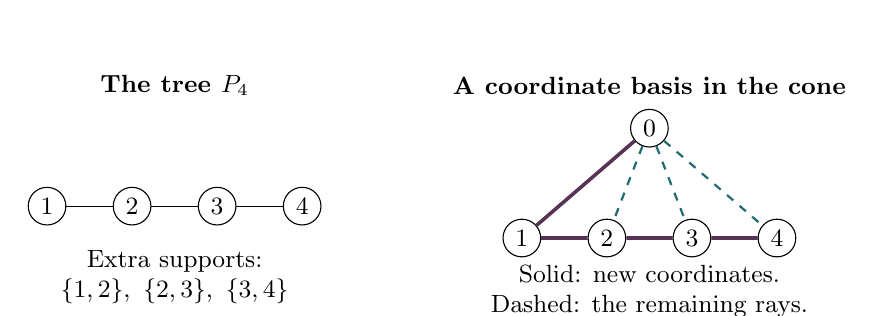
\begin{tikzpicture}[scale=0.9, every node/.style={font=\small},
  vertex/.style={circle,draw=black,fill=white,inner sep=2.2pt},
  selected/.style={draw=inkplum,line width=1.3pt},
  omitted/.style={draw=inkteal,dashed,line width=0.8pt}]
\begin{scope}
 \node[font=\small\bfseries] at (1.8,2.15) {The tree $P_4$};
 \foreach \i in {1,2,3,4} {\node[vertex] (a\i) at ({1.2*(\i-1)},0.45) {$\i$};}
 \draw (a1)--(a2)--(a3)--(a4);
 \node[align=center] at (1.8,-0.55) {Extra supports:\\$\{1,2\},\ \{2,3\},\ \{3,4\}$};
\end{scope}
\begin{scope}[xshift=6.7cm]
 \node[font=\small\bfseries] at (1.8,2.15) {A coordinate basis in the cone};
 \node[vertex] (o) at (1.8,1.55) {$0$};
 \foreach \i in {1,2,3,4} {\node[vertex] (b\i) at ({1.2*(\i-1)},0.0) {$\i$};}
 \draw[selected] (o)--(b1)--(b2)--(b3)--(b4);
 \draw[omitted] (o)--(b2) (o)--(b3) (o)--(b4);
 \node[align=center] at (1.8,-0.75) {Solid: new coordinates.\\Dashed: the remaining rays.};
\end{scope}
\end{tikzpicture}
\caption{A tree support graph becomes a hypergraph after a linear change of variables. With $z_1=y_1$, $z_2=y_2-y_1$, $z_3=y_3-y_2$, $z_4=y_4-y_3$, the omitted spokes are $y_2=z_1+z_2$, $y_3=z_1+z_2+z_3$ and $y_4=z_1+z_2+z_3+z_4$, with supports $\{1,2\}$, $\{1,2,3\}$, $\{1,2,3,4\}$.}
\label{lv:fig:path-presentation}
\end{figure}

\begin{example}[P$_3$ continued]
For P$_3$ the cone has $B(P_3)=8$ spanning trees. In the numerical example of \S1 the five rays are $x_1,x_2,x_3,Q_{12}=x_1-2x_2,Q_{23}=3x_2-4x_3$. The bases $\{x_1,x_2,x_3\}$, $\{x_2,x_3,Q_{12}\}$, $\{x_1,x_2,Q_{23}\}$ and $\{x_2,Q_{12},Q_{23}\}$ give a path-shaped support graph. The other four bases, among them $\{x_1,Q_{12},Q_{23}\}$ used in Example~\ref{lv:ex:P3}, give the hypergraph $\{\{1,2\},\{1,2,3\}\}$. So $q(P_3)=2$, in agreement with \cite[\S4.2]{lv:K2025}.
\end{example}

\subsection{Three counting questions}

Write $B(T)$ for the number of coordinate bases (unordered, up to scaling) and $q(T)$ for the number of nonisomorphic hypergraphs $\mathcal H_S$. By the matrix-tree theorem,
\begin{equation}
 B(T)=\tau(\Cone(T))=\det(I_n+L_T),
 \qquad
 B(P_n)=F_{2n},\quad B(K_{1,n-1})=2^{n-2}(n+1),
 \label{lv:eq:basis-count}
\end{equation}
where $L_T$ is the graph Laplacian; these are classical \cite{lv:RS2024}. Retaining the order of coordinates multiplies $B(T)$ by $n!$, and retaining the numerical scalings gives infinitely many changes.

\paragraph{Relation to the source's counts.}
The procedure quoted in \S1.3, applied to a generic tree system, produces exactly the hypergraphs $\mathcal H_S$. Read in this way, the per-tree entries of \cite[Table~7]{lv:K2025} are the numbers $q(T)$, and this agrees with Table~\ref{lv:tab:counts} for every $n\leq8$, as multisets, since the source lists trees in its own order (Section~\ref{lv:sec:verification}). We do not prove that the general class of LV systems attached to $\mathcal H_S$ consists only of $S$-presentations of tree systems; its parameter count could in principle be larger \lab{open}. The identification with the source's equivalence classes uses only the procedure as quoted. We note that, at $n=6$, the source's Table~7 lists $2,8,5,18,21,30$ while its Appendix Figure~15 labels the trees $2,8,8,18,21,30$. Our computation and Corollary~\ref{lv:cor:stars} (the double star with $a=b=2$ has $q=5$) agree with Table~7.

\section{When two presentations have isomorphic supports}
\label{lv:sec:orbits}

A graph automorphism of $G$ permutes spanning trees, but the right symmetry group is larger. In plain terms: two coordinate choices give isomorphic support pictures exactly when some relabelling of the Darboux rays that preserves all linear dependencies carries one choice to the other.

\begin{proposition}[Hypergraphs and basis orbits]
\label{lv:prop:orbit-equivalence}
For spanning trees $S,S'$ of $G$,
\(
 \mathcal H_S\cong\mathcal H_{S'}
\)
if and only if $\gamma(S)=S'$ for some $\gamma\in\Aut M(G)$. Consequently
\begin{equation}
 q(T)=\bigl|\Aut M(G)\backslash\mathcal B(M(G))\bigr|,
 \label{lv:eq:orbit-count}
\end{equation}
where $\mathcal B(M(G))$ is the set of spanning trees.
\end{proposition}

\begin{proof}
A matroid automorphism sends the unique circuit in $S\cup\{e\}$ to the unique circuit in $S'\cup\{\gamma(e)\}$, and hence sends $\pi_S(e)$ to $\pi_{S'}(\gamma(e))$. Conversely, let $\phi:S\to S'$ be a hypergraph isomorphism. The non-basis edges are determined by their (distinct) fundamental supports, so $\phi$ extends uniquely to a permutation $\gamma$ of $E(G)$ with $\pi_{S'}(\gamma(e))=\phi(\pi_S(e))$. Over $\mathbb F_2$, the fundamental cycles $\{e\}\cup\pi_S(e)$ form a basis of the cycle space (the edge sets in which every vertex has even degree). The map $\gamma$ carries this basis to the corresponding basis for $S'$, hence preserves the cycle space and its minimal nonzero supports, which are the circuits. So $\gamma\in\Aut M(G)$.
\end{proof}

This is the binary-matroid fact that fundamental supports determine a representation $[I\mid A]$ over $\mathbb F_2$ \cite[\S6.4]{lv:Oxley2011}. It shows why forgetting the signs in \eqref{lv:eq:path-expansion} loses nothing for this question.

\begin{theorem}[Matroid automorphisms]
\label{lv:thm:automorphisms}
Let $\ell(T)$ be the number of leaves. For $n\geq3$,
\begin{equation}
 \Aut M(\Cone(T))\cong (C_2)^{\ell(T)}\rtimes\Aut(T),
 \label{lv:eq:automorphism-group}
\end{equation}
where the factor $C_2$ at a leaf $v$ with neighbour $u$ swaps $s_v$ and $r_{uv}$, and $\Aut(T)$ acts through its action on cone edges. For $n=2$ the matroid is $U_{2,3}$ and the group is $S_3$.
\end{theorem}

\begin{proof}
Every matroid automorphism permutes the triangles \eqref{lv:eq:triangles}, preserving intersections. It therefore induces an automorphism of $L(T)$, hence, by Lemma~\ref{lv:lem:line-graph}, a unique automorphism of $T$. This gives a homomorphism $\Aut M(G)\to\Aut(T)$. It restricts to the identity on graph automorphisms of $T$ acting on cone edges, which gives a splitting.

Let $\gamma$ be in the kernel, so $\gamma$ fixes every triangle. For an internal vertex $v$, the spoke $s_v$ is the unique common element of the at least two triangles at $v$, so it is fixed. A tree edge between internal vertices is then the third element of a triangle with two fixed elements. In a pendant triangle $\{s_u,s_v,r_{uv}\}$ with leaf $v$, only $s_v$ and $r_{uv}$ can move, and they can only be exchanged. So the kernel is contained in $(C_2)^{\ell(T)}$.

Every such swap is a matroid automorphism. The $n-1$ triangles form a basis of the binary cycle space, because each contains its own tree edge and no other triangle contains it. A swap preserves the set of triangles, hence their span, hence all circuits. The swaps commute, and $\Aut(T)$ permutes them through its action on leaves.
\end{proof}

In matroid language, $s_v$ and $r_{uv}$ form a \emph{series pair}: the leaf $v$ has degree two in the cone. Elements of a series class can be permuted by matroid automorphisms. This is Whitney's 2-isomorphism phenomenon \cite{lv:Whitney1933}, \cite[\S5.3]{lv:Oxley2011}, and it is why $\Aut M(G)$ exceeds the graph automorphism group. On normalised forms the swap is realised by $y_v\mapsto y_u-y_v$. This is a symmetry of the arrangement, not of the differential equation.

\section{Reduction to decorated rooted forests of the core}
\label{lv:sec:core}

Let $n\geq3$, let $H=T[\{v:\deg_T v\geq2\}]$ be the (nonempty, connected) tree of internal vertices, let $L_x$ be the set of leaves of $T$ attached to $x\in V(H)$, and let $\lambda_x=|L_x|$. Then $\Aut(H,\lambda)$ is the group of automorphisms of $H$ that preserve $\lambda$ exactly.

\begin{definition}
A \emph{decorated rooted forest} of $(H,\lambda)$ is a spanning forest $F\subseteq E(H)$ with one root chosen in each component and a type in $\{0,1\}$ at each root. Type $1$ is allowed at $x$ only if $\lambda_x>0$.
\end{definition}

\begin{lemma}[Quotient structure]
\label{lv:lem:quotient}
Let $\Gamma=\Aut M(G)$ and let $N\leq\Gamma$ be generated by the leaf swaps and by the automorphisms of $T$ that fix every internal vertex.
\begin{enumerate}
\item The automorphisms of $T$ fixing $V(H)$ pointwise are exactly the products of permutations of each $L_x$. Restriction gives a surjection $\Aut(T)\to\Aut(H,\lambda)$ with this kernel.
\item $N=(C_2)^{\ell(T)}\rtimes\prod_x\mathrm{Sym}(L_x)$ is normal in $\Gamma$, and $\Gamma/N\cong\Aut(H,\lambda)$.
\item There is a surjection $\Phi$ from spanning trees of $G$ to decorated rooted forests such that $\Phi(S)=\Phi(S')$ if and only if $S'\in N S$, and $\Phi(\gamma S)=\bar\gamma\,\Phi(S)$ for $\gamma\in\Gamma$ with image $\bar\gamma\in\Aut(H,\lambda)$.
\end{enumerate}
\end{lemma}

\begin{proof}
(i) An automorphism fixing $V(H)$ maps each leaf to a leaf with the same neighbour, and any such permutation is an automorphism. An automorphism of $T$ preserves internal vertices and the number of leaves at each, so it restricts to $\Aut(H,\lambda)$. Conversely, $\sigma\in\Aut(H,\lambda)$ extends by choosing bijections $L_x\to L_{\sigma(x)}$, which exist because $\lambda_x=\lambda_{\sigma(x)}$.

(ii) $N$ is the kernel of the composite of the surjections $\Gamma\to\Aut(T)$ (Theorem~\ref{lv:thm:automorphisms}) and $\Aut(T)\to\Aut(H,\lambda)$.

(iii) Let $S$ be a spanning tree of $G$. A leaf $v\in L_x$ has only the two cone edges $s_v$ and $r_{xv}$, and at least one of them lies in $S$. If exactly one does, $v$ is a pendant vertex of $S$; delete it and its edge. If both do, $v$ has degree two in $S$; replace the path $x-v-0$ by a single \emph{virtual edge} from $x$ to $0$ labelled $v$. The result is a spanning tree of the multigraph $H^+$, obtained from $H$ by adding a vertex $0$ joined to each $x$ by the spoke $s_x$ and by one virtual edge for each $v\in L_x$. Removing $0$ from a spanning tree of $H^+$ leaves a spanning forest $F$ of $H$ in which each component is joined to $0$ by exactly one edge: at least one by connectivity, at most one by acyclicity. Let $\Phi(S)$ be $F$, rooted at the endpoint of that edge, with type $0$ for a spoke and type $1$ for a virtual edge. The construction is reversible once one records, in addition, which leaf realises each type-$1$ root and which edge is kept at each other leaf. So $\Phi$ is surjective, and its fibres are exactly the possible values of this additional data.

A leaf swap at an unused leaf changes which edge is kept, and a swap at a leaf realising a root fixes $S$. A permutation of $L_x$ changes only the additional data. So $\Phi$ is constant on $N$-orbits. Conversely, if $\Phi(S)=\Phi(S')$, each $x$ realises at most one type-$1$ root, because $x$ is the root of at most one component. A permutation of each $L_x$ moves the realising leaves of $S$ to those of $S'$, and swaps at the remaining leaves then match the kept edges. So $S'\in NS$. Finally, for $\tau\in\Aut(T)$ the construction is natural, $\Phi(\tau S)=\tau|_H\,\Phi(S)$, and every $\gamma\in\Gamma$ is a product of an element of $N$ and an element of $\Aut(T)$.
\end{proof}

\begin{theorem}[Core-forest classification]
\label{lv:thm:core}
For $n\geq3$, the nonisomorphic support hypergraphs of a generic $T$-system are in bijection with the $\Aut(H,\lambda)$-orbits of decorated rooted forests of $(H,\lambda)$.
\end{theorem}

\begin{proof}
By Proposition~\ref{lv:prop:orbit-equivalence} we need the $\Gamma$-orbits of spanning trees. By Lemma~\ref{lv:lem:quotient}(iii), $\Phi$ identifies $N$-orbits with decorated forests, compatibly with $\Gamma\to\Gamma/N\cong\Aut(H,\lambda)$. Hence $\Gamma$-orbits of spanning trees correspond to $\Aut(H,\lambda)$-orbits of decorated forests.
\end{proof}

The number of root types at $x$ is $w_x=1+\mathbf 1_{\lambda_x>0}$, not $1+\lambda_x$: the identity of the realising leaf is removed by $N$.

\begin{corollary}[A determinant]
\label{lv:cor:core-determinant}
The number of decorated rooted forests is $r(T)=\det(L_H+\operatorname{diag}(w_x))$. If $\Aut(H,\lambda)$ is trivial, then $q(T)=r(T)$.
\end{corollary}

\begin{proof}
Join a new vertex $0$ to each $x$ by $w_x$ parallel edges. Spanning trees of the resulting multigraph are decorated rooted forests, as in the proof of Lemma~\ref{lv:lem:quotient}. The reduced Laplacian at $0$ is $L_H+\operatorname{diag}(w)$, so the matrix-tree theorem applies; equivalently, use the weighted matrix-forest theorem \cite{lv:CS1997}.
\end{proof}

\begin{corollary}[Stars and double stars]
\label{lv:cor:stars}
For $n\geq3$, $q(K_{1,n-1})=2$. If $T$ is a double star whose two internal vertices carry $a,b\geq1$ leaves, then $q(T)=5$ if $a=b$ and $q(T)=8$ if $a\neq b$.
\end{corollary}

\begin{proof}
For a star the core is one vertex with two root types. For a double star the core is an edge $xy$ with $w_x=w_y=2$. Without the core edge there are $2\cdot2$ type assignments; with it there are $2$ choices of root and $2$ of type, so $r=8=\det\begin{pmatrix}3&-1\\-1&3\end{pmatrix}$. If $a\neq b$, $\Aut(H,\lambda)$ is trivial. If $a=b$, the reflection splits the first four objects into the orbits $\{00\},\{11\},\{01,10\}$ and the second four into two orbits, giving $5$.
\end{proof}

\begin{example}[P$_4$ worked through]
The path $1-2-3-4$ is the double star with $a=b=1$. Its cone has $B(P_4)=F_8=21$ spanning trees. The leaf swaps at $1$ and $4$ act freely on the choices made at unused leaves, and the eight decorated forests of the core edge $\{2,3\}$ fall into $5$ reflection orbits. So $q(P_4)=5$. For instance, the basis of Figure~\ref{lv:fig:path-presentation} uses both edges at the leaf $1$ (a type-$1$ root at $2$) and contains the core edge.
\end{example}

These examples show why dividing $B(T)$ by a group order does not give $q(T)$: stabilisers vary.

\section{Closed counts for paths and caterpillars}
\label{lv:sec:paths}

For weights $w_1,\dots,w_k$ let $R(w_1,\dots,w_k)=\det(L_{P_k}+\operatorname{diag}(w))$, the number of decorated rooted forests of a path whose $i$th vertex has $w_i$ root types, with $R()=1$.

\begin{theorem}[Path count]
\label{lv:thm:path-count}
For $n\geq2$,
\begin{equation}
 q(P_n)=\frac{F_{2n-2}+F_{n-1}}{2}.
 \label{lv:eq:path-count}
\end{equation}
\end{theorem}

\begin{proof}
For $n=2$ the cone is a triangle and $q=1$; for $n=3$ the core is one vertex with two types, so $q=2$. Both agree with \eqref{lv:eq:path-count}. Let $n\geq4$ and $m=n-2$. The core is $P_m$ with weights $(2,1,\dots,1,2)$, and its only nontrivial colour-preserving automorphism is the reflection.

\emph{All forests.} The matrix has diagonal $3$ and off-diagonal $-1$, so its determinant $D_m$ satisfies $D_0=1$, $D_1=3$, $D_m=3D_{m-1}-D_{m-2}$, whence $D_m=F_{2m+2}$. (The value $D_1$ is auxiliary; the case $n=3$ was treated directly.)

\emph{One-sided count.} Let $A_j=R(2,1,\dots,1)$ on $j$ vertices, with $A_0=1$. Expanding at the weight-one end gives $A_1=2$ and $A_j=3A_{j-1}-A_{j-2}$, so $A_j=F_{2j+1}$.

\emph{Fixed forests.} If $m=2r$, an invariant forest cannot contain the central edge: the central component would be invariant with no fixed vertex at which to put its root. The forest is then determined by its left half, so there are $A_r=F_{m+1}$ fixed forests. If $m=2r+1$, the component of the middle vertex is a symmetric interval rooted there, with type $0$ because the middle core vertex has no leaves. If $j$ vertices lie to its left, the left part is an arbitrary decorated forest on $j$ vertices, so there are $\sum_{j=0}^rA_j=\sum_{j=0}^rF_{2j+1}=F_{2r+2}=F_{m+1}$ fixed forests.

Burnside's lemma gives $q=(F_{2m+2}+F_{m+1})/2=(F_{2n-2}+F_{n-1})/2$.
\end{proof}

The values for $n=2,3,\dots$ are $1,2,5,12,30,76,195,504,1309,3410,\dots$. This sequence, with its Fibonacci formula, appears in the OEIS as A051450 (with index $n-1$), where it counts positive rational knots \cite{lv:OEIS}; we do not construct a bijection. The path does not maximise $q$: at $n=7$ some tree has $q=79>q(P_7)=76$.

A \emph{caterpillar} is a tree whose internal vertices induce a path $H=v_1-\dots-v_m$; for $m\geq2$ the end vertices carry leaves, $\lambda_1,\lambda_m\geq1$. Paths ($\lambda=(1,0,\dots,0,1)$) and double stars ($m=2$) are examples.

\begin{theorem}[Caterpillar count]
\label{lv:thm:caterpillar}
Let $T$ be a caterpillar with $m\geq2$, leaf counts $\lambda_1,\dots,\lambda_m$ and weights $w_i=1+\mathbf 1_{\lambda_i>0}$. If $(\lambda_1,\dots,\lambda_m)$ is not a palindrome, then $q(T)=R(w_1,\dots,w_m)$. If it is a palindrome, then $q(T)=\tfrac12\bigl(R(w_1,\dots,w_m)+\mathrm{Fix}\bigr)$, where
\[
 \mathrm{Fix}=
 \begin{cases}
 R(w_1,\dots,w_{m/2}), & m\text{ even},\\[2pt]
 w_c\sum_{j=0}^{(m-1)/2}R(w_1,\dots,w_j), & m\text{ odd},\ c=\tfrac{m+1}2.
 \end{cases}
\]
\end{theorem}

\begin{proof}
$\Aut(H,\lambda)$ is trivial unless $\lambda$ is a palindrome, in which case it is generated by the reflection. Apply Theorem~\ref{lv:thm:core}, Corollary~\ref{lv:cor:core-determinant} and Burnside's lemma. The fixed forests are counted as in Theorem~\ref{lv:thm:path-count}. For $m$ even, the central edge is absent and the left half is arbitrary. For $m$ odd, the middle vertex roots a symmetric interval with any of its $w_c$ types, and the part to its left is an arbitrary decorated forest on $j$ vertices. Reflection preserves types because it preserves $\lambda$.
\end{proof}

For $\lambda=(1,0,\dots,0,1)$ this recovers Theorem~\ref{lv:thm:path-count}, and for $m=2$ it recovers Corollary~\ref{lv:cor:stars}. The formula agrees with the exact enumeration for all $142$ caterpillars with at least two internal vertices (paths included) and $n\leq10$ (Section~\ref{lv:sec:verification}).

\section{Consequences}
\label{lv:sec:consequences}

\subsection{Recognising a tree system}

\begin{theorem}[Recognition]
\label{lv:thm:recognition}
A homogeneous quadratic system $\dot x=f(x)$ on $\K^n$ is linearly conjugate to a $T$-system with matrix in $U_T$ if and only if its homogeneous linear Darboux rays form a finite set of exactly $2n-1$ elements whose matroid is isomorphic to $M(\Cone(T))$.
\end{theorem}

\begin{proof}
Necessity follows from Theorem~\ref{lv:thm:complete} and the invariance of the Darboux set under conjugacy. Conversely, let $\psi$ be a matroid isomorphism from the rays to $E(\Cone T)$. The rays corresponding to spokes form a basis; use their forms $z_1,\dots,z_n$ as coordinates. The ray $\psi^{-1}(r_{uv})$ lies in a three-element circuit with $z_u$ and $z_v$, and it is proportional to neither, because the rays are distinct. So its form is supported exactly on $\{u,v\}$, with both coefficients nonzero. By Lemma~\ref{lv:lem:coordinate-criterion} the system is LV in $z$. By Lemma~\ref{lv:lem:dp-test} its matrix satisfies \eqref{lv:eq:LT-equations}, so it lies in $L_T$. Its complete ray set has the form (ii) of Theorem~\ref{lv:thm:complete}, so $\Delta_T\neq0$.
\end{proof}

This answers a practical question: given a numerical LV matrix, decide whether it is secretly a generic tree system, and find the tree. One computes its finitely many linear Darboux rays with Lemma~\ref{lv:lem:dp-test}, checks that there are $2n-1$ of them, and reads $T$ from the intersection graph of the three-element circuits. No elimination over candidate hypergraphs is needed.

\begin{example}[Van der Kamp's 13-parameter system] \lab{exploratory}
The source presents a 5-component superintegrable LV system with 13 parameters, its matrix (34), with supports $\{1,2\},\{1,3\},\{2,4\},\{1,2,5\}$, and calls it ``a new superintegrable LV-system that is not equivalent to a tree-system'' \cite[\S4.4]{lv:K2025}. At five random integer parameter points, our exact computation finds exactly $9=2n-1$ rays, of rank $5$, with four three-element circuits, the same numbers as for a tree system. The matroid is nevertheless not isomorphic to the cone matroid of any tree on five vertices: its circuit-size profile is $\{3{:}4,4{:}3,5{:}3,6{:}1\}$, while the three cone profiles are $\{3{:}4,4{:}4,5{:}2\}$, $\{3{:}4,4{:}3,5{:}2,6{:}1\}$ and $\{3{:}4,4{:}6\}$. By Theorem~\ref{lv:thm:recognition}, at these points the system is not conjugate to any generic tree system. For general parameters of the family this is supported by the sample points only. Conjugacy to a special tree system (outside $U_T$) is not excluded by this test.
\end{example}

\subsection{Kahan discretisation}

For $\dot x=f(x)$ homogeneous quadratic, let $\mathcal B$ be the symmetric bilinear map with $\mathcal B(x,x)=f(x)$. Kahan's discretisation with step $h$ \cite{lv:Kahan,lv:KahanLi1997,lv:CMOQ2013} is the birational map $x\mapsto x'$ defined by $x'-x=h\,\mathcal B(x,x')$. For LV systems, $\mathcal B(x,y)_i=\tfrac12(x_i(Ay)_i+y_i(Ax)_i)$.

\begin{proposition}[Darboux polynomials of Kahan maps]
\label{lv:prop:kahan}
If $P$ is a linear Darboux polynomial of $f$ with cofactor $C$, then
\[
 P(x')\bigl(1-\tfrac h2C(x)\bigr)=P(x)\bigl(1+\tfrac h2C(x')\bigr).
\]
Kahan's discretisation commutes with linear changes of variables. Hence for $A\in U_T$, every ray in $\mathcal D_T$ is a discrete Darboux polynomial of the Kahan map, and every coordinate presentation of Theorem~\ref{lv:thm:all-coordinates} is a presentation of the Kahan map in which all $2n-1$ rays are discrete Darboux polynomials.
\end{proposition}

\begin{proof}
Polarising the identity $P(f(x))=P(x)C(x)$ gives $P(\mathcal B(x,y))=\tfrac12(P(x)C(y)+P(y)C(x))$. Hence $P(x')-P(x)=hP(\mathcal B(x,x'))=\tfrac h2(P(x)C(x')+P(x')C(x))$, which rearranges to the claim. If $z=Mx$, the bilinear map of the transformed field is $M\mathcal B(M^{-1}z,M^{-1}z')$, so the Kahan relation is transformed into the Kahan relation.
\end{proof}

The preservation of affine Darboux polynomials by Kahan's method is stated in \cite{lv:CEMOQTK2019} (Theorem~1 in \S2 of arXiv:1902.04715, whose proof is announced there for a later paper); tree systems and their Kahan maps are studied in \cite{lv:QTMK2023b}. We do not claim that the Kahan map has no further linear discrete Darboux polynomials \lab{open}.

\subsection{Positivity and other notions of equivalence}

\begin{remark}[Positivity]
\label{lv:rem:positivity}
In population dynamics and chemical reaction networks the variables are positive, and the natural equivalences preserve the positive orthant (compare the linear conjugacy of reaction networks, which uses positive diagonal maps and permutations \cite{lv:JS2011}). A linear map with $B(\mathbb R^n_{>0})=\mathbb R^n_{>0}$ has $B\geq0$ and $B^{-1}\geq0$ entrywise, so it is a monomial matrix. Among the presentations of Theorem~\ref{lv:thm:all-coordinates}, only the original one, $S=\{s_v\}$, has this form, up to positive scaling and reordering. So, within orthant-preserving linear changes, the tree support of a generic tree system is its only presentation. The hypergraph presentations of \cite{lv:K2025} are genuinely non-positive.
\end{remark}

\begin{remark}[Quasi-monomial equivalence]
\label{lv:rem:quasi}
Generalised LV systems are often compared by quasi-monomial transformations $x\mapsto x^M$ \cite{lv:Brenig1988,lv:HBF1997}. These do not map linear forms to linear forms, so the Darboux arrangement is not an invariant for them. Whether tree rigidity has a quasi-monomial analogue is open \lab{open}. The skew-symmetric LV systems studied up to linear isomorphism in \cite{lv:EKV2022} form a different class: LV-preserving linear changes need not preserve skew-symmetry \cite{lv:KMQ2026}.
\end{remark}

\section{Exact computations}
\label{lv:sec:verification}

The proofs above hold for every finite tree. The computations are finite checks of these proofs and of their interpretation. All arithmetic is exact (Python integers and rationals; \texttt{sympy} for symbolic identities), and the outputs are deterministic (Section~\ref{lv:sec:data}).

\begin{enumerate}
\item \emph{Cone bases and orbits} (\texttt{verify.py}). All $94$ trees with $2\leq n\leq9$: Darboux supports at two exact generic points per tree ($63\,580$ support subsets), the $120\,479$ cone bases, $\det(I+L_T)$, and the orbit counts under the generators of Theorem~\ref{lv:thm:automorphisms}. For $n\leq8$ the multisets of counts equal those of \cite[Table~7]{lv:K2025}.
\item \emph{Direct isomorphism check} (\texttt{verify\_hypergraphs.py}). For all $13$ trees with $n\leq6$ (986 bases), the hypergraphs $\mathcal H_S$ are canonicalised under all $n!$ permutations, without using the group of Theorem~\ref{lv:thm:automorphisms}. The counts agree.
\item \emph{Core model} (\texttt{lv\_core\_count.py}). The decorated-forest orbit count for all $200$ trees with $n\leq10$, generated by a separate tree generator. This is an algorithmically distinct enumeration, written in the same project, not an independent replication.
\item \emph{Extensions} (\texttt{verify\_extensions.py}). Lemma~\ref{lv:lem:cofactor} on all ray pairs for $n\leq7$. Theorem~\ref{lv:thm:one-sided} for $n\leq6$ over all bases; for $n\leq5$ also directly against all labelled trees $T'$. Theorem~\ref{lv:thm:complete}(ii)$\Rightarrow$(i) on $2000$ small-integer points per tree for $n\leq5$ (no mismatch; for some trees few of these points are generic). Proposition~\ref{lv:prop:strata} at $428$ constructed single-factor points for $n\leq6$, and the pencil when $d_{u\to v}=d_{v\to u}=0$. Proposition~\ref{lv:prop:intersection} in all $288$ cases with $n\leq7$. Proposition~\ref{lv:prop:tangent} (dimension $2n-1$) for $n\leq6$. Theorem~\ref{lv:thm:caterpillar} for all caterpillars with $n\leq10$. Also Example~\ref{lv:ex:P3}, the Kahan identity (symbolically), Remark~\ref{lv:rem:constant-b}, Remark~\ref{lv:rem:positivity} for P$_4$, and the exploratory example of \S8.1.
\end{enumerate}

\begin{table}[htbp]
\centering
\begin{tabular}{rrrrr}
\toprule
$n$ & trees & $q(K_{1,n-1})$ & $q(P_n)$ & maximum of $q(T)$\\
\midrule
2 & 1   & 1 & 1    & 1\\
3 & 1   & 2 & 2    & 2\\
4 & 2   & 2 & 5    & 5\\
5 & 3   & 2 & 12   & 12\\
6 & 6   & 2 & 30   & 30\\
7 & 11  & 2 & 76   & 79\\
8 & 23  & 2 & 195  & 207\\
9 & 47  & 2 & 504  & 545\\
10& 106 & 2 & 1309 & 1467\\
\bottomrule
\end{tabular}
\caption{Support-hypergraph counts \lab{exact computation}. The rows $n\leq9$ come from both the cone-basis and the core enumerations; $n=10$ from the core enumeration only. For $n\leq8$ the per-tree multisets agree with \cite[Table~7]{lv:K2025}. Per-tree values are in the data files.}
\label{lv:tab:counts}
\end{table}

\section{Limits and open problems}
\label{lv:sec:limits}

\begin{itemize}
\item \lab{open} The Darboux sets at points where two or more factors of $\Delta_T$ vanish, and conjugacies between two special systems of different families beyond Proposition~\ref{lv:prop:intersection}.
\item \lab{open} Whether the general class attached to each $\mathcal H_S$ (in the source's sense) coincides with the $S$-presentations of tree systems, which would make the identification with \cite[Table~7]{lv:K2025} a theorem for all $n$ rather than a consequence of the source's stated procedure.
\item \lab{open} Structural formulas for $q(T)$ beyond caterpillars, and the trees maximising $q(T)$ for each $n$.
\item \lab{open} Higher-degree Darboux polynomials, quasi-monomial equivalence, and completeness of the linear Darboux set of Kahan maps.
\end{itemize}

\section*{Statements}
\label{lv:sec:data}

\paragraph{Use of AI tools.}
This work was carried out with substantial assistance from AI systems (large language models), which were used for mathematical exploration, drafting of proofs and text, writing of verification code, and checking. The author reviewed the arguments and takes responsibility for the content. Any errors are the author's.

\paragraph{Data and code availability.}
The verification code and its outputs accompany this article. The command \texttt{python3 verify\_all.py} regenerates every output and compares it byte for byte with the archived files. The archive is deposited at Zenodo, \href{https://doi.org/10.5281/zenodo.23564794}{doi:10.5281/zenodo.23564794} (version 1.0.0-candidate), and at \url{https://github.com/ipitchford/lotka-volterra-tree-presentations}.

\paragraph{Competing interests and funding.}
None.

\begin{thebibliography}{99}\small

\bibitem{lv:AM2026} T.~Abe, S.~Murai, Vector fields of graphic arrangements and face rings of simplicial posets, preprint (2026), \href{https://arxiv.org/abs/2608.06767}{arXiv:2608.06767}.

\bibitem{lv:Bog2008} O.~I. Bogoyavlenskij, Integrable Lotka--Volterra systems, \emph{Regul. Chaotic Dyn.} \textbf{13}(6) (2008) 543--556. \href{https://doi.org/10.1134/S1560354708060051}{doi:10.1134/S1560354708060051}.

\bibitem{lv:Brenig1988} L.~Brenig, Complete factorisation and analytic solutions of generalized Lotka--Volterra equations, \emph{Phys. Lett. A} \textbf{133}(7--8) (1988) 378--382. \href{https://doi.org/10.1016/0375-9601(88)90920-6}{doi:10.1016/0375-9601(88)90920-6}.

\bibitem{lv:CL2000} L.~Cair\'o, J.~Llibre, Darboux integrability for 3D Lotka--Volterra systems, \emph{J. Phys. A: Math. Gen.} \textbf{33}(12) (2000) 2395--2406. \href{https://doi.org/10.1088/0305-4470/33/12/307}{doi:10.1088/0305-4470/33/12/307}.

\bibitem{lv:CEMOQTK2019} E.~Celledoni, C.~Evripidou, D.~I. McLaren, B.~Owren, G.~R.~W. Quispel, B.~K. Tapley, P.~H. van der Kamp, Using discrete Darboux polynomials to detect and determine preserved measures and integrals of rational maps, \emph{J. Phys. A: Math. Theor.} \textbf{52}(31) (2019) 31LT01. \href{https://doi.org/10.1088/1751-8121/ab294b}{doi:10.1088/1751-8121/ab294b}; \href{https://arxiv.org/abs/1902.04715}{arXiv:1902.04715}.

\bibitem{lv:CMOQ2013} E.~Celledoni, R.~I. McLachlan, B.~Owren, G.~R.~W. Quispel, Geometric properties of Kahan's method, \emph{J. Phys. A: Math. Theor.} \textbf{46}(2) (2013) 025201. \href{https://doi.org/10.1088/1751-8113/46/2/025201}{doi:10.1088/1751-8113/46/2/025201}.

\bibitem{lv:CS1997} P.~Chebotarev, E.~Shamis, Matrix-forest theorems, unpublished manuscript (1994--1997), \href{https://arxiv.org/abs/math/0602575}{arXiv:math/0602575}.

\bibitem{lv:CD2009} Y.~T. Christodoulides, P.~A. Damianou, Darboux polynomials for Lotka--Volterra systems in three dimensions, \emph{J. Nonlinear Math. Phys.} \textbf{16}(3) (2009) 339--354. \href{https://doi.org/10.1142/S1402925109000261}{doi:10.1142/S1402925109000261}.

\bibitem{lv:EKV2022} C.~A. Evripidou, P.~Kassotakis, P.~Vanhaecke, Morphisms and automorphisms of skew-symmetric Lotka--Volterra systems, \emph{J. Phys. A: Math. Theor.} \textbf{55}(32) (2022) 325201. \href{https://doi.org/10.1088/1751-8121/ac7e90}{doi:10.1088/1751-8121/ac7e90}; \href{https://arxiv.org/abs/2010.16180}{arXiv:2010.16180}.

\bibitem{lv:HBF1997} B.~Hern\'andez-Bermejo, V.~Fair\'en, Lotka--Volterra representation of general nonlinear systems, \emph{Math. Biosci.} \textbf{140}(1) (1997) 1--32. \href{https://doi.org/10.1016/S0025-5564(96)00131-9}{doi:10.1016/S0025-5564(96)00131-9}.

\bibitem{lv:JS2011} M.~D. Johnston, D.~Siegel, Linear conjugacy of chemical reaction networks, \emph{J. Math. Chem.} \textbf{49}(7) (2011) 1263--1282. \href{https://doi.org/10.1007/s10910-011-9817-4}{doi:10.1007/s10910-011-9817-4}.

\bibitem{lv:Jung1966} H.~A. Jung, Zu einem Isomorphiesatz von H.~Whitney f\"ur Graphen, \emph{Math. Ann.} \textbf{164}(3) (1966) 270--271. \href{https://doi.org/10.1007/BF01360250}{doi:10.1007/BF01360250}.

\bibitem{lv:Kahan} W.~Kahan, Unconventional numerical methods for trajectory calculations, unpublished lecture notes (1993).

\bibitem{lv:KahanLi1997} W.~Kahan, R.-C. Li, Unconventional schemes for a class of ordinary differential equations---with applications to the Korteweg--de Vries equation, \emph{J. Comput. Phys.} \textbf{134}(2) (1997) 316--331. \href{https://doi.org/10.1006/jcph.1997.5710}{doi:10.1006/jcph.1997.5710}.

\bibitem{lv:K2025} P.~H. van der Kamp, Hypergraphs and Lotka--Volterra systems with linear Darboux polynomials, \emph{J. Dyn. Diff. Equat.} \textbf{38}(3) (2026) 1331--1352 (online 2025). \href{https://doi.org/10.1007/s10884-025-10446-2}{doi:10.1007/s10884-025-10446-2}; \href{https://arxiv.org/abs/2411.18264v4}{arXiv:2411.18264v4}.

\bibitem{lv:QTMK2023b} P.~H. van der Kamp, R.~I. McLachlan, D.~I. McLaren, G.~R.~W. Quispel, Measure preservation and integrals for Lotka--Volterra tree-systems and their Kahan discretisation, \emph{J. Comput. Dyn.} \textbf{11}(4) (2024) 468--484. \href{https://doi.org/10.3934/jcd.2024011}{doi:10.3934/jcd.2024011}; \href{https://arxiv.org/abs/2309.05979}{arXiv:2309.05979}.

\bibitem{lv:KMQ2026} P.~H. van der Kamp, D.~I. McLaren, G.~R.~W. Quispel, Liouville integrable Lotka--Volterra systems, \emph{Open Commun. Nonlinear Math. Phys.} (2026), ocnmp:18125. \href{https://doi.org/10.46298/ocnmp.18125}{doi:10.46298/ocnmp.18125}; \href{https://arxiv.org/abs/2604.01743}{arXiv:2604.01743}.

\bibitem{lv:KQM2024} P.~H. van der Kamp, G.~R.~W. Quispel, D.~I. McLaren, Trees and superintegrable Lotka--Volterra families, \emph{Math. Phys. Anal. Geom.} \textbf{27}(4) (2024) 25. \href{https://doi.org/10.1007/s11040-024-09496-7}{doi:10.1007/s11040-024-09496-7}; \href{https://arxiv.org/abs/2311.15169}{arXiv:2311.15169}.

\bibitem{lv:MO2001} J.~Moulin Ollagnier, Liouvillian integration of the Lotka--Volterra system, \emph{Qual. Theory Dyn. Syst.} \textbf{2}(2) (2001) 307--358. \href{https://doi.org/10.1007/BF02969345}{doi:10.1007/BF02969345}.

\bibitem{lv:OEIS} OEIS Foundation Inc., The On-Line Encyclopedia of Integer Sequences, sequence \href{https://oeis.org/A051450}{A051450}. Accessed 22 October 2026.

\bibitem{lv:Oxley2011} J.~Oxley, \emph{Matroid Theory}, 2nd ed., Oxford University Press, 2011. \href{https://doi.org/10.1093/acprof:oso/9780198566946.001.0001}{doi:10.1093/acprof:oso/9780198566946.001.0001}.

\bibitem{lv:PR2019} N.~Proudfoot, E.~Ramos, Functorial invariants of trees and their cones, \emph{Selecta Math. (N.S.)} \textbf{25}(4) (2019) 62. \href{https://doi.org/10.1007/s00029-019-0509-4}{doi:10.1007/s00029-019-0509-4}; \href{https://arxiv.org/abs/1903.10592}{arXiv:1903.10592}.

\bibitem{lv:QTMK2023} G.~R.~W. Quispel, B.~K. Tapley, D.~I. McLaren, P.~H. van der Kamp, Linear Darboux polynomials for Lotka--Volterra systems, trees and superintegrable families, \emph{J. Phys. A: Math. Theor.} \textbf{56}(31) (2023) 315201. \href{https://doi.org/10.1088/1751-8121/ace0e9}{doi:10.1088/1751-8121/ace0e9}; \href{https://arxiv.org/abs/2303.00229}{arXiv:2303.00229}.

\bibitem{lv:RS2024} V.~Reiner, D.~Smith, Sandpile groups for cones over trees, \emph{Res. Math. Sci.} \textbf{11}(4) (2024) 59. \href{https://doi.org/10.1007/s40687-024-00471-w}{doi:10.1007/s40687-024-00471-w}; \href{https://arxiv.org/abs/2402.15453}{arXiv:2402.15453}.

\bibitem{lv:Toh2015} \c{S}.~O. Toh\v{a}neanu, Projective duality of arrangements with quadratic logarithmic vector fields, \emph{Discrete Math.} \textbf{339}(1) (2016) 54--61. \href{https://doi.org/10.1016/j.disc.2015.07.004}{doi:10.1016/j.disc.2015.07.004}; \href{https://arxiv.org/abs/1405.2122}{arXiv:1405.2122}.

\bibitem{lv:Whitney1932} H.~Whitney, Congruent graphs and the connectivity of graphs, \emph{Amer. J. Math.} \textbf{54}(1) (1932) 150--168. \href{https://doi.org/10.2307/2371086}{doi:10.2307/2371086}.

\bibitem{lv:Whitney1933} H.~Whitney, 2-isomorphic graphs, \emph{Amer. J. Math.} \textbf{55} (1933) 245--254. \href{https://doi.org/10.2307/2371127}{doi:10.2307/2371127}.

\end{thebibliography}
\end{document}
